% Options for packages loaded elsewhere
\PassOptionsToPackage{unicode}{hyperref}
\PassOptionsToPackage{hyphens}{url}
%
\documentclass[
]{article}
\title{575 Final Project: Data Analysis}
\author{Lizzie, Suhaib, Emma}
\date{2021-11-03}

\usepackage{amsmath,amssymb}
\usepackage{lmodern}
\usepackage{iftex}
\ifPDFTeX
  \usepackage[T1]{fontenc}
  \usepackage[utf8]{inputenc}
  \usepackage{textcomp} % provide euro and other symbols
\else % if luatex or xetex
  \usepackage{unicode-math}
  \defaultfontfeatures{Scale=MatchLowercase}
  \defaultfontfeatures[\rmfamily]{Ligatures=TeX,Scale=1}
\fi
% Use upquote if available, for straight quotes in verbatim environments
\IfFileExists{upquote.sty}{\usepackage{upquote}}{}
\IfFileExists{microtype.sty}{% use microtype if available
  \usepackage[]{microtype}
  \UseMicrotypeSet[protrusion]{basicmath} % disable protrusion for tt fonts
}{}
\makeatletter
\@ifundefined{KOMAClassName}{% if non-KOMA class
  \IfFileExists{parskip.sty}{%
    \usepackage{parskip}
  }{% else
    \setlength{\parindent}{0pt}
    \setlength{\parskip}{6pt plus 2pt minus 1pt}}
}{% if KOMA class
  \KOMAoptions{parskip=half}}
\makeatother
\usepackage{xcolor}
\IfFileExists{xurl.sty}{\usepackage{xurl}}{} % add URL line breaks if available
\IfFileExists{bookmark.sty}{\usepackage{bookmark}}{\usepackage{hyperref}}
\hypersetup{
  pdftitle={575 Final Project: Data Analysis},
  pdfauthor={Lizzie, Suhaib, Emma},
  hidelinks,
  pdfcreator={LaTeX via pandoc}}
\urlstyle{same} % disable monospaced font for URLs
\usepackage[margin=1in]{geometry}
\usepackage{color}
\usepackage{fancyvrb}
\newcommand{\VerbBar}{|}
\newcommand{\VERB}{\Verb[commandchars=\\\{\}]}
\DefineVerbatimEnvironment{Highlighting}{Verbatim}{commandchars=\\\{\}}
% Add ',fontsize=\small' for more characters per line
\usepackage{framed}
\definecolor{shadecolor}{RGB}{248,248,248}
\newenvironment{Shaded}{\begin{snugshade}}{\end{snugshade}}
\newcommand{\AlertTok}[1]{\textcolor[rgb]{0.94,0.16,0.16}{#1}}
\newcommand{\AnnotationTok}[1]{\textcolor[rgb]{0.56,0.35,0.01}{\textbf{\textit{#1}}}}
\newcommand{\AttributeTok}[1]{\textcolor[rgb]{0.77,0.63,0.00}{#1}}
\newcommand{\BaseNTok}[1]{\textcolor[rgb]{0.00,0.00,0.81}{#1}}
\newcommand{\BuiltInTok}[1]{#1}
\newcommand{\CharTok}[1]{\textcolor[rgb]{0.31,0.60,0.02}{#1}}
\newcommand{\CommentTok}[1]{\textcolor[rgb]{0.56,0.35,0.01}{\textit{#1}}}
\newcommand{\CommentVarTok}[1]{\textcolor[rgb]{0.56,0.35,0.01}{\textbf{\textit{#1}}}}
\newcommand{\ConstantTok}[1]{\textcolor[rgb]{0.00,0.00,0.00}{#1}}
\newcommand{\ControlFlowTok}[1]{\textcolor[rgb]{0.13,0.29,0.53}{\textbf{#1}}}
\newcommand{\DataTypeTok}[1]{\textcolor[rgb]{0.13,0.29,0.53}{#1}}
\newcommand{\DecValTok}[1]{\textcolor[rgb]{0.00,0.00,0.81}{#1}}
\newcommand{\DocumentationTok}[1]{\textcolor[rgb]{0.56,0.35,0.01}{\textbf{\textit{#1}}}}
\newcommand{\ErrorTok}[1]{\textcolor[rgb]{0.64,0.00,0.00}{\textbf{#1}}}
\newcommand{\ExtensionTok}[1]{#1}
\newcommand{\FloatTok}[1]{\textcolor[rgb]{0.00,0.00,0.81}{#1}}
\newcommand{\FunctionTok}[1]{\textcolor[rgb]{0.00,0.00,0.00}{#1}}
\newcommand{\ImportTok}[1]{#1}
\newcommand{\InformationTok}[1]{\textcolor[rgb]{0.56,0.35,0.01}{\textbf{\textit{#1}}}}
\newcommand{\KeywordTok}[1]{\textcolor[rgb]{0.13,0.29,0.53}{\textbf{#1}}}
\newcommand{\NormalTok}[1]{#1}
\newcommand{\OperatorTok}[1]{\textcolor[rgb]{0.81,0.36,0.00}{\textbf{#1}}}
\newcommand{\OtherTok}[1]{\textcolor[rgb]{0.56,0.35,0.01}{#1}}
\newcommand{\PreprocessorTok}[1]{\textcolor[rgb]{0.56,0.35,0.01}{\textit{#1}}}
\newcommand{\RegionMarkerTok}[1]{#1}
\newcommand{\SpecialCharTok}[1]{\textcolor[rgb]{0.00,0.00,0.00}{#1}}
\newcommand{\SpecialStringTok}[1]{\textcolor[rgb]{0.31,0.60,0.02}{#1}}
\newcommand{\StringTok}[1]{\textcolor[rgb]{0.31,0.60,0.02}{#1}}
\newcommand{\VariableTok}[1]{\textcolor[rgb]{0.00,0.00,0.00}{#1}}
\newcommand{\VerbatimStringTok}[1]{\textcolor[rgb]{0.31,0.60,0.02}{#1}}
\newcommand{\WarningTok}[1]{\textcolor[rgb]{0.56,0.35,0.01}{\textbf{\textit{#1}}}}
\usepackage{graphicx}
\makeatletter
\def\maxwidth{\ifdim\Gin@nat@width>\linewidth\linewidth\else\Gin@nat@width\fi}
\def\maxheight{\ifdim\Gin@nat@height>\textheight\textheight\else\Gin@nat@height\fi}
\makeatother
% Scale images if necessary, so that they will not overflow the page
% margins by default, and it is still possible to overwrite the defaults
% using explicit options in \includegraphics[width, height, ...]{}
\setkeys{Gin}{width=\maxwidth,height=\maxheight,keepaspectratio}
% Set default figure placement to htbp
\makeatletter
\def\fps@figure{htbp}
\makeatother
\setlength{\emergencystretch}{3em} % prevent overfull lines
\providecommand{\tightlist}{%
  \setlength{\itemsep}{0pt}\setlength{\parskip}{0pt}}
\setcounter{secnumdepth}{-\maxdimen} % remove section numbering
\usepackage{booktabs}
\usepackage{siunitx}
\newcolumntype{d}{S[input-symbols = ()]}
\usepackage{longtable}
\usepackage{array}
\usepackage{multirow}
\usepackage{wrapfig}
\usepackage{float}
\usepackage{colortbl}
\usepackage{pdflscape}
\usepackage{tabu}
\usepackage{threeparttable}
\usepackage{threeparttablex}
\usepackage[normalem]{ulem}
\usepackage{makecell}
\usepackage{xcolor}
\ifLuaTeX
  \usepackage{selnolig}  % disable illegal ligatures
\fi

\begin{document}
\maketitle

{
\setcounter{tocdepth}{2}
\tableofcontents
}
\hypertarget{load-packages}{%
\section{Load packages}\label{load-packages}}

\begin{Shaded}
\begin{Highlighting}[]
\FunctionTok{library}\NormalTok{(tidyverse)}
\FunctionTok{library}\NormalTok{(haven)}
\FunctionTok{library}\NormalTok{(ggplot2)}
\FunctionTok{library}\NormalTok{(here)}
\FunctionTok{library}\NormalTok{(jtools)}
\FunctionTok{library}\NormalTok{(lme4)}
\FunctionTok{library}\NormalTok{(lmerTest)}
\FunctionTok{library}\NormalTok{(glmmTMB)}
\FunctionTok{library}\NormalTok{(modelsummary)}
\FunctionTok{theme\_set}\NormalTok{(jtools}\SpecialCharTok{::}\FunctionTok{theme\_apa}\NormalTok{())}
\end{Highlighting}
\end{Shaded}

\hypertarget{load-data}{%
\section{Load Data}\label{load-data}}

\hypertarget{import-data}{%
\subsection{Import Data}\label{import-data}}

\begin{Shaded}
\begin{Highlighting}[]
\CommentTok{\# Read in the data}
\NormalTok{df.hatch }\OtherTok{\textless{}{-}} \FunctionTok{read\_sav}\NormalTok{(}\FunctionTok{here}\NormalTok{(}\StringTok{"HATCH 09.29.21.sav"}\NormalTok{))}
\end{Highlighting}
\end{Shaded}

\hypertarget{tidy-data}{%
\subsection{Tidy Data}\label{tidy-data}}

\begin{Shaded}
\begin{Highlighting}[]
\CommentTok{\# Subset Variables}
\NormalTok{df.mlm }\OtherTok{\textless{}{-}}\NormalTok{ df.hatch }\SpecialCharTok{\%\textgreater{}\%}
  \FunctionTok{select}\NormalTok{(}\FunctionTok{c}\NormalTok{(CoupID,                                }\CommentTok{\# Couple ID}
           
           \CommentTok{\# Couple Level                         \#\# COUPLE \#\#}
\NormalTok{           DelMod, ModeofDeliverySpecific,        }\CommentTok{\# Delivery Method}
\NormalTok{           GesAgeWk,                              }\CommentTok{\# Gestational age}
\NormalTok{           Bb.sex,                                }\CommentTok{\# Baby sex}
           
           \CommentTok{\# Person Level                         \#\# PERSON \#\#}
           \FunctionTok{contains}\NormalTok{(}\StringTok{"pnAge"}\NormalTok{),                     }\CommentTok{\# Parent age}
           \FunctionTok{contains}\NormalTok{(}\StringTok{"Ethn"}\NormalTok{),                      }\CommentTok{\# Parent ethnicity}
           \FunctionTok{contains}\NormalTok{(}\StringTok{"Educ"}\NormalTok{),                      }\CommentTok{\# Parent level of education}
           \FunctionTok{contains}\NormalTok{(}\StringTok{"peritot"}\NormalTok{),                   }\CommentTok{\# BEQ (birth stress)}
           
           \CommentTok{\# Time Level                           \#\# TIME \#\#}
\NormalTok{           bage3pp}\FloatTok{.1}\NormalTok{, bage6pp, bage12pp}\FloatTok{.1}\NormalTok{,        }\CommentTok{\# Baby age}
           \FunctionTok{contains}\NormalTok{(}\StringTok{"PSI\_t"}\NormalTok{),                     }\CommentTok{\# Parenting Stress}
              \FunctionTok{contains}\NormalTok{(}\StringTok{"PSIt"}\NormalTok{),}
              \FunctionTok{contains}\NormalTok{(}\StringTok{"PSI.t"}\NormalTok{)}
\NormalTok{           ))   }

\CommentTok{\# Rename Variables}
\FunctionTok{colnames}\NormalTok{(df.mlm) }\OtherTok{\textless{}{-}} \FunctionTok{c}\NormalTok{(}\StringTok{"CoupID"}\NormalTok{,}
                      
                      \CommentTok{\# Couple Level}
                      \StringTok{"DelMeth"}\NormalTok{, }\StringTok{"DelMeth.Specific"}\NormalTok{,}
                      \StringTok{"GestationAge"}\NormalTok{,}
                      \StringTok{"BabySex"}\NormalTok{,}
                      
                      \CommentTok{\# Person Level}
                      \StringTok{"age.mom"}\NormalTok{, }\StringTok{"age.dad"}\NormalTok{,}
                      \StringTok{"ethnicity.mom"}\NormalTok{, }\StringTok{"ethnicity.dad"}\NormalTok{,}
                      \StringTok{"education.mom"}\NormalTok{, }\StringTok{"education.dad"}\NormalTok{,}
                      \StringTok{"beq.mom"}\NormalTok{, }\StringTok{"beq.dad"}\NormalTok{,}
                      
                      \CommentTok{\# Time Level}
                      \StringTok{"BabyAge.3"}\NormalTok{, }\StringTok{"BabyAge.6"}\NormalTok{, }\StringTok{"BabyAge.12"}\NormalTok{,}
                      \StringTok{"PSI.3.mom"}\NormalTok{, }\StringTok{"PSI.12.mom"}\NormalTok{, }\StringTok{"PSI.12.dad"}\NormalTok{,}
                          \StringTok{"PSI.3.dad"}\NormalTok{, }\StringTok{"PSI.6.dad"}\NormalTok{,}
                          \StringTok{"PSI.6.mom"}
\NormalTok{                      )}

\CommentTok{\# Reorder PSI Variables}
\NormalTok{df.mlm }\OtherTok{\textless{}{-}}\NormalTok{ df.mlm }\SpecialCharTok{\%\textgreater{}\%}
  \FunctionTok{relocate}\NormalTok{(}\FunctionTok{c}\NormalTok{(}\StringTok{"PSI.3.mom"}\NormalTok{, }\StringTok{"PSI.3.dad"}\NormalTok{,}
             \StringTok{"PSI.6.mom"}\NormalTok{, }\StringTok{"PSI.6.dad"}\NormalTok{,}
             \StringTok{"PSI.12.mom"}\NormalTok{, }\StringTok{"PSI.12.dad"}\NormalTok{),}
           \AttributeTok{.after =}\NormalTok{ BabyAge}\FloatTok{.12}\NormalTok{)}
\end{Highlighting}
\end{Shaded}

\hypertarget{wide-to-long}{%
\subsection{Wide to Long}\label{wide-to-long}}

\begin{Shaded}
\begin{Highlighting}[]
\CommentTok{\# Person{-}Level and Time{-}Level Variables}
\NormalTok{df.long1 }\OtherTok{\textless{}{-}}\NormalTok{ df.mlm }\SpecialCharTok{\%\textgreater{}\%}
  \CommentTok{\# Parent{-}level variables}
  \FunctionTok{pivot\_longer}\NormalTok{(}
    \AttributeTok{cols =}\NormalTok{ age.mom}\SpecialCharTok{:}\NormalTok{beq.dad,}
    \AttributeTok{names\_to =} \FunctionTok{c}\NormalTok{(}\StringTok{".value"}\NormalTok{, }\StringTok{"parent"}\NormalTok{),}
    \AttributeTok{names\_pattern =} \StringTok{"(age|ethnicity|education|beq).(mom|dad)"}\NormalTok{,}
    \AttributeTok{names\_transform =} \FunctionTok{list}\NormalTok{(}\AttributeTok{parent =}\NormalTok{ as.factor)}
\NormalTok{  ) }\SpecialCharTok{\%\textgreater{}\%}
  \CommentTok{\# Assign participant IDs}
  \FunctionTok{mutate}\NormalTok{(}\AttributeTok{PersonID =} \FunctionTok{seq}\NormalTok{(}\DecValTok{1}\SpecialCharTok{:}\DecValTok{200}\NormalTok{)) }\SpecialCharTok{\%\textgreater{}\%}
  \CommentTok{\# Time{-}level variables}
  \FunctionTok{pivot\_longer}\NormalTok{(}
    \AttributeTok{cols =}\NormalTok{ BabyAge}\FloatTok{.3}\SpecialCharTok{:}\NormalTok{BabyAge}\FloatTok{.12}\NormalTok{,}
    \AttributeTok{names\_to =} \FunctionTok{c}\NormalTok{(}\StringTok{".value"}\NormalTok{, }\StringTok{"time"}\NormalTok{),}
    \AttributeTok{names\_pattern =} \StringTok{"(BabyAge).(3|6|12)"}\NormalTok{,}
    \AttributeTok{names\_transform =} \FunctionTok{list}\NormalTok{(}\AttributeTok{time =}\NormalTok{ as.integer)}
\NormalTok{  ) }\SpecialCharTok{\%\textgreater{}\%}
  \CommentTok{\# Remove PSI variables}
  \FunctionTok{select}\NormalTok{(}\SpecialCharTok{{-}}\FunctionTok{starts\_with}\NormalTok{(}\StringTok{"PSI"}\NormalTok{))}

\CommentTok{\# PSI Variable}
\NormalTok{df.long2 }\OtherTok{\textless{}{-}}\NormalTok{ df.mlm }\SpecialCharTok{\%\textgreater{}\%}
  \FunctionTok{pivot\_longer}\NormalTok{(}
    \AttributeTok{cols =}\NormalTok{ PSI.}\FloatTok{3.}\NormalTok{mom}\SpecialCharTok{:}\NormalTok{PSI.}\FloatTok{12.}\NormalTok{dad,}
    \AttributeTok{names\_to =} \FunctionTok{c}\NormalTok{(}\StringTok{".value"}\NormalTok{, }\StringTok{"time"}\NormalTok{, }\StringTok{"parent"}\NormalTok{),}
    \AttributeTok{names\_pattern =} \StringTok{"(PSI).(3|6|12).(mom|dad)"}\NormalTok{,}
    \AttributeTok{names\_transform =} \FunctionTok{list}\NormalTok{(}\AttributeTok{time =}\NormalTok{ as.integer, }\AttributeTok{parent =}\NormalTok{ as.factor)}
\NormalTok{  ) }\SpecialCharTok{\%\textgreater{}\%}
  \CommentTok{\# Remove variables in \textasciigrave{}df.long1\textasciigrave{} that aren\textquotesingle{}t identifying variables}
  \FunctionTok{select}\NormalTok{(}\FunctionTok{c}\NormalTok{(CoupID, time, parent, PSI))}


\CommentTok{\# Combine Data Frames}
\NormalTok{df.long }\OtherTok{\textless{}{-}} \FunctionTok{left\_join}\NormalTok{(df.long1, df.long2, }\AttributeTok{by =} \FunctionTok{c}\NormalTok{(}\StringTok{"CoupID"}\NormalTok{, }\StringTok{"parent"}\NormalTok{, }\StringTok{"time"}\NormalTok{)) }\SpecialCharTok{\%\textgreater{}\%}
  \CommentTok{\# Move identifying variable}
  \FunctionTok{relocate}\NormalTok{(}\FunctionTok{c}\NormalTok{(PersonID, parent, time), }\AttributeTok{.after =}\NormalTok{ CoupID) }\SpecialCharTok{\%\textgreater{}\%}
  \CommentTok{\# Remove funky formatting}
  \FunctionTok{mutate}\NormalTok{(}\AttributeTok{beq =} \FunctionTok{na\_if}\NormalTok{(beq, }\SpecialCharTok{{-}}\FloatTok{97.450}\NormalTok{))}
\end{Highlighting}
\end{Shaded}

\hypertarget{density-plots}{%
\section{Density Plots}\label{density-plots}}

\begin{Shaded}
\begin{Highlighting}[]
\FunctionTok{ggplot}\NormalTok{(}\AttributeTok{data =}\NormalTok{ df.long, }\FunctionTok{aes}\NormalTok{(}\AttributeTok{x =}\NormalTok{ PSI)) }\SpecialCharTok{+}
  \FunctionTok{geom\_density}\NormalTok{() }\SpecialCharTok{+}
  \FunctionTok{facet\_grid}\NormalTok{(parent}\SpecialCharTok{\textasciitilde{}}\NormalTok{time) }\SpecialCharTok{+}
  \FunctionTok{labs}\NormalTok{(}\AttributeTok{x =} \StringTok{"Parenting Stress (PSI)"}\NormalTok{, }\AttributeTok{y =} \StringTok{""}\NormalTok{)}
\end{Highlighting}
\end{Shaded}

\begin{verbatim}
## Warning: Removed 98 rows containing non-finite values (stat_density).
\end{verbatim}

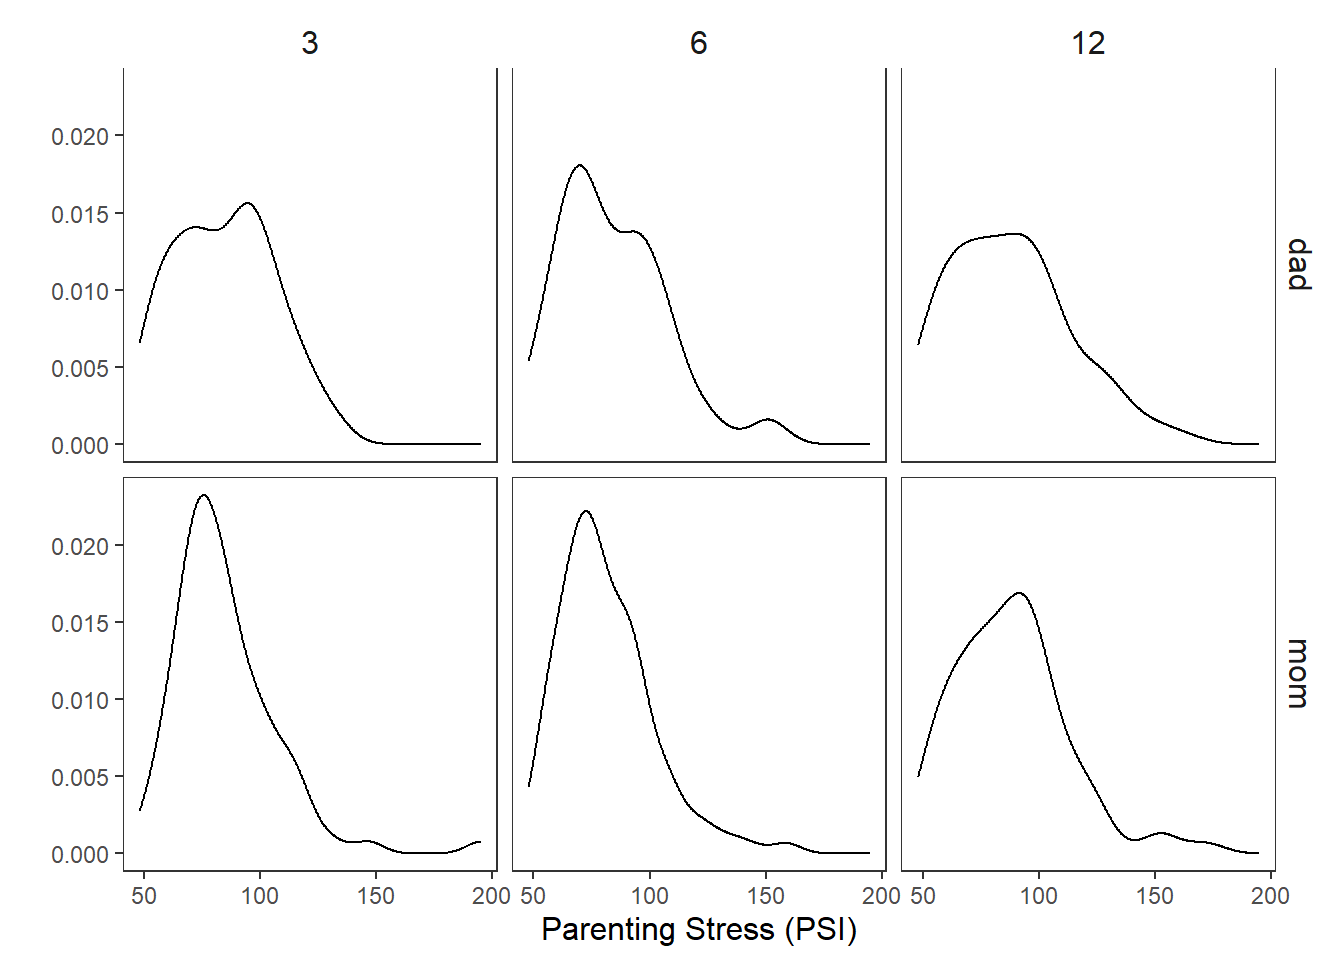
\includegraphics{final_project_analyses_files/figure-latex/plot-density-1.pdf}

\begin{Shaded}
\begin{Highlighting}[]
\FunctionTok{ggplot}\NormalTok{(}\AttributeTok{data =}\NormalTok{ df.long, }\FunctionTok{aes}\NormalTok{(}\AttributeTok{x =}\NormalTok{ beq)) }\SpecialCharTok{+} 
  \FunctionTok{geom\_density}\NormalTok{() }\SpecialCharTok{+} 
  \FunctionTok{facet\_wrap}\NormalTok{(}\SpecialCharTok{\textasciitilde{}}\NormalTok{parent) }\SpecialCharTok{+}
  \FunctionTok{labs}\NormalTok{(}\AttributeTok{x =} \StringTok{"Birthing Stress (BEQ)"}\NormalTok{, }\AttributeTok{y =} \StringTok{""}\NormalTok{)}
\end{Highlighting}
\end{Shaded}

\begin{verbatim}
## Warning: Removed 45 rows containing non-finite values (stat_density).
\end{verbatim}

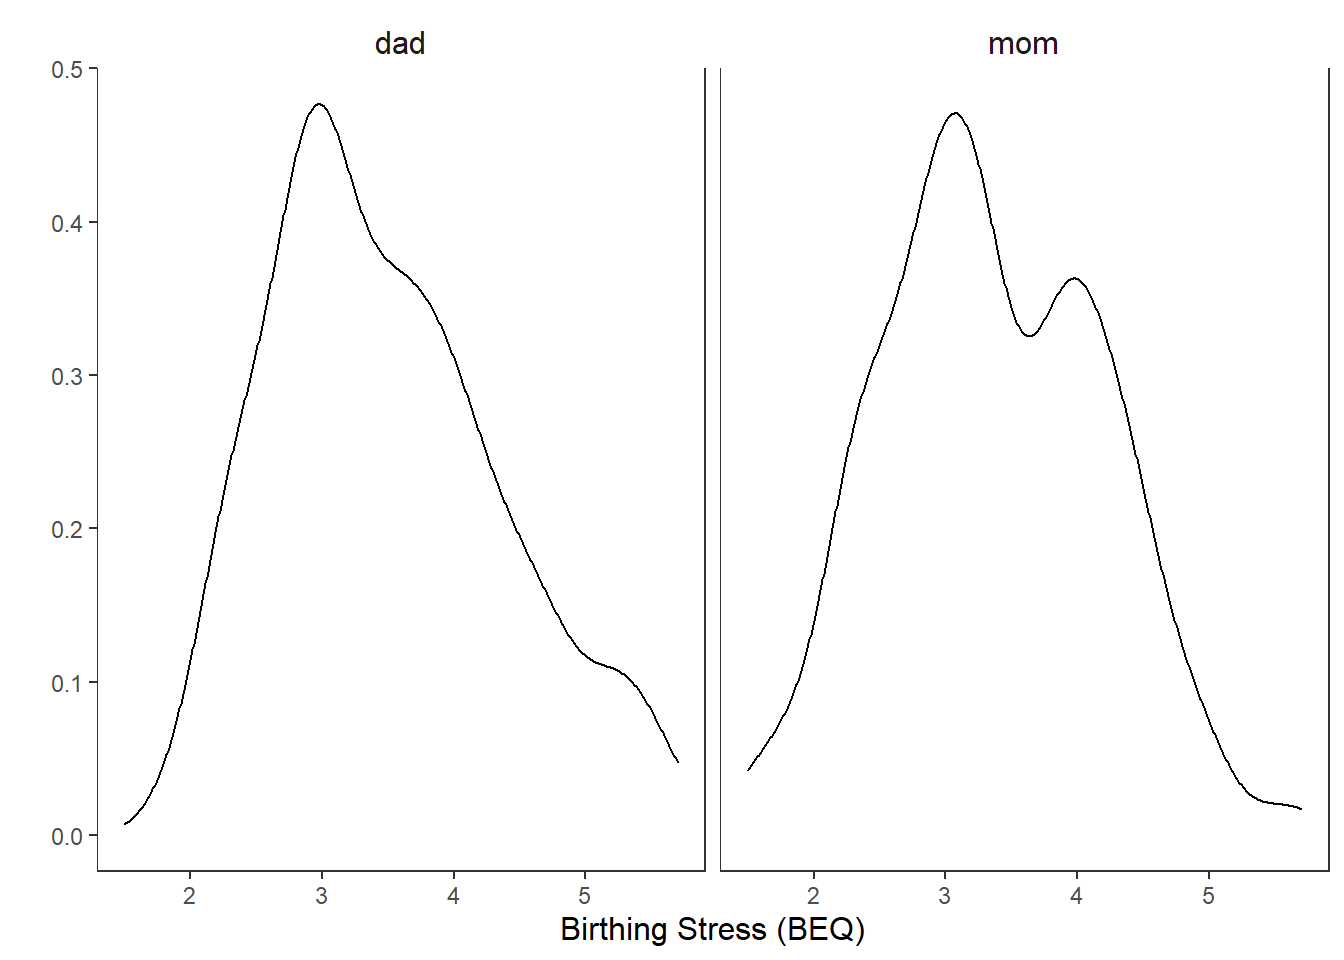
\includegraphics{final_project_analyses_files/figure-latex/plot-density-2.pdf}

\begin{Shaded}
\begin{Highlighting}[]
\FunctionTok{ggplot}\NormalTok{(}\AttributeTok{data =} \FunctionTok{na.omit}\NormalTok{(}\FunctionTok{distinct}\NormalTok{(df.long, CoupID, }\AttributeTok{.keep\_all =}\NormalTok{ T)), }
       \FunctionTok{aes}\NormalTok{(}\AttributeTok{x =} \FunctionTok{as.factor}\NormalTok{(DelMeth), }
           \AttributeTok{fill =} \FunctionTok{as.factor}\NormalTok{(DelMeth.Specific))) }\SpecialCharTok{+} 
  \FunctionTok{geom\_bar}\NormalTok{(}\AttributeTok{position =} \StringTok{"stack"}\NormalTok{, }\AttributeTok{color =} \StringTok{"black"}\NormalTok{) }\SpecialCharTok{+} 
  \FunctionTok{scale\_x\_discrete}\NormalTok{(}\AttributeTok{labels =} \FunctionTok{c}\NormalTok{(}\StringTok{"Vaginal"}\NormalTok{, }\StringTok{"C{-}Section"}\NormalTok{)) }\SpecialCharTok{+} 
  \FunctionTok{scale\_fill\_discrete}\NormalTok{(}\AttributeTok{labels =} \FunctionTok{c}\NormalTok{(}\StringTok{"Natural Vaginal"}\NormalTok{, }\StringTok{"Medicated Vaginal"}\NormalTok{, }\StringTok{"Unplanned C{-}Section"}\NormalTok{, }\StringTok{"Planned C{-}Section"}\NormalTok{)) }\SpecialCharTok{+}
  \FunctionTok{labs}\NormalTok{(}\AttributeTok{x =} \StringTok{"Delivery Method"}\NormalTok{, }\AttributeTok{y =} \StringTok{""}\NormalTok{)}
\end{Highlighting}
\end{Shaded}

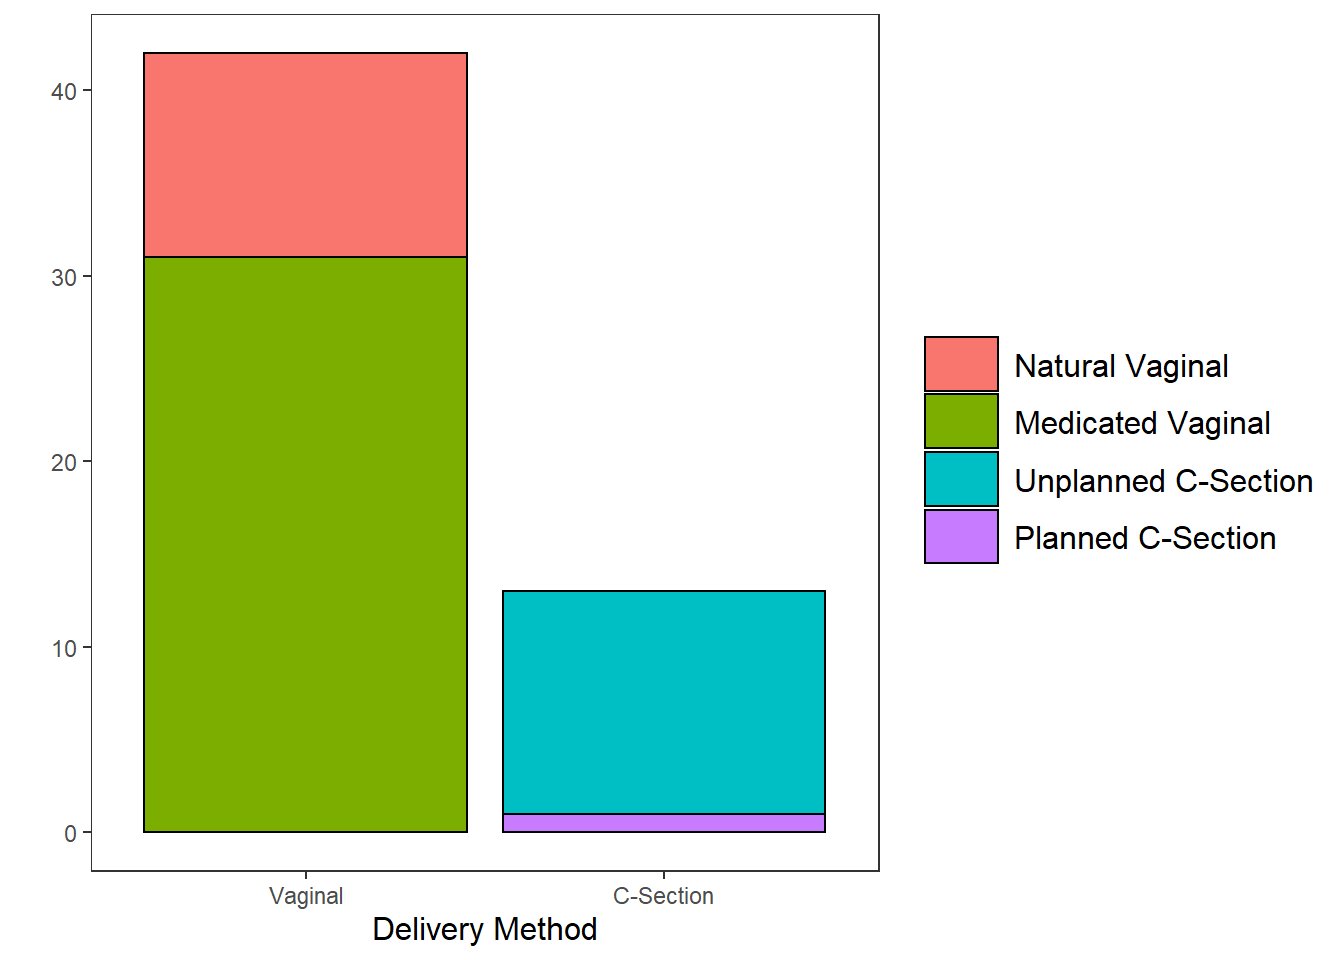
\includegraphics{final_project_analyses_files/figure-latex/plot-density-3.pdf}

\hypertarget{data-processing}{%
\subsection{Data Processing}\label{data-processing}}

\begin{Shaded}
\begin{Highlighting}[]
\CommentTok{\#scaling and decomposing of variables}
\NormalTok{df\_scaled }\OtherTok{\textless{}{-}}\NormalTok{ df.long }\SpecialCharTok{\%\textgreater{}\%} \FunctionTok{mutate}\NormalTok{(}\AttributeTok{log\_psi =} \FunctionTok{scale}\NormalTok{(}\FunctionTok{log}\NormalTok{(PSI))) }\SpecialCharTok{\%\textgreater{}\%}
  \FunctionTok{group\_by}\NormalTok{(CoupID) }\SpecialCharTok{\%\textgreater{}\%} \FunctionTok{mutate}\NormalTok{(}\AttributeTok{beq\_cm =} \FunctionTok{mean}\NormalTok{(beq)) }\SpecialCharTok{\%\textgreater{}\%} \FunctionTok{ungroup}\NormalTok{() }\SpecialCharTok{\%\textgreater{}\%} \FunctionTok{mutate}\NormalTok{(}\AttributeTok{beq\_cmc =}\NormalTok{ beq }\SpecialCharTok{{-}}\NormalTok{ beq\_cm)}
\end{Highlighting}
\end{Shaded}

\hypertarget{models}{%
\subsection{Models}\label{models}}

\hypertarget{model-equation}{%
\subsubsection{Model Equation:}\label{model-equation}}

Nomenclature: j: Couples i: persons t: time intervals

\begin{align}
(\#eq:m2)
<!-- $$  -->
psi_{tij} = \gamma_{000} + \gamma_{100} \cdot TIME_{tij} + \gamma_{010}\cdot beq^{cmc}_{ij} + u_{0i0} + \gamma_{001}\cdot beq^{cm}_{j} + \gamma_{002}\cdot DelMeth_j + \gamma_{003}\cdot DelMeth\cdot beq^{cm}_j + u_{00j} + e_{tij}
<!-- $$ -->
\end{align}

\hypertarget{modelling}{%
\subsubsection{Modelling}\label{modelling}}

\begin{Shaded}
\begin{Highlighting}[]
\NormalTok{m0 }\OtherTok{\textless{}{-}} \FunctionTok{lmer}\NormalTok{(PSI }\SpecialCharTok{\textasciitilde{}} \DecValTok{1} \SpecialCharTok{+}\NormalTok{ (time}\SpecialCharTok{|}\NormalTok{CoupID), }\AttributeTok{data=}\NormalTok{df\_scaled)}
\FunctionTok{ranova}\NormalTok{(m0) }\CommentTok{\#not significant!}
\end{Highlighting}
\end{Shaded}

\begin{verbatim}
## ANOVA-like table for random-effects: Single term deletions
## 
## Model:
## PSI ~ (time | CoupID)
##                         npar  logLik    AIC    LRT Df Pr(>Chisq)
## <none>                     5 -2189.3 4388.6                     
## time in (time | CoupID)    3 -2191.2 4388.5 3.8782  2     0.1438
\end{verbatim}

\begin{Shaded}
\begin{Highlighting}[]
\CommentTok{\#random slope insignificant for Couples and does not converge for Persons}
\end{Highlighting}
\end{Shaded}

The random slope on the couple level is not significant, so it will not
be included in the model. Note, that the model did not converge for
person-level random slopes, which is why they have been excluded for
now, however, they are planned to be included in future versions.

\begin{Shaded}
\begin{Highlighting}[]
\NormalTok{m1 }\OtherTok{\textless{}{-}} \FunctionTok{glmmTMB}\NormalTok{(PSI }\SpecialCharTok{\textasciitilde{}}\NormalTok{ time }\SpecialCharTok{+}\NormalTok{ beq\_cmc  }\SpecialCharTok{+}\NormalTok{ DelMeth}\SpecialCharTok{*}\NormalTok{beq\_cm }\SpecialCharTok{+}\NormalTok{ (}\DecValTok{1}\SpecialCharTok{|}\NormalTok{PersonID) }\SpecialCharTok{+}\NormalTok{ (}\DecValTok{1}\SpecialCharTok{|}\NormalTok{CoupID), }\AttributeTok{data =}\NormalTok{ df\_scaled)}
\FunctionTok{summary}\NormalTok{(m1) }\CommentTok{\#robust se estimation (faster than brms)}
\end{Highlighting}
\end{Shaded}

\begin{verbatim}
##  Family: gaussian  ( identity )
## Formula:          
## PSI ~ time + beq_cmc + DelMeth * beq_cm + (1 | PersonID) + (1 |      CoupID)
## Data: df_scaled
## 
##      AIC      BIC   logLik deviance df.resid 
##   3300.1   3335.6  -1641.1   3282.1      372 
## 
## Random effects:
## 
## Conditional model:
##  Groups   Name        Variance Std.Dev.
##  PersonID (Intercept) 118.4    10.88   
##  CoupID   (Intercept) 169.7    13.03   
##  Residual             182.3    13.50   
## Number of obs: 381, groups:  PersonID, 147; CoupID, 74
## 
## Dispersion estimate for gaussian family (sigma^2):  182 
## 
## Conditional model:
##                Estimate Std. Error z value Pr(>|z|)    
## (Intercept)    74.35352   11.74448   6.331 2.44e-10 ***
## time            0.24808    0.19832   1.251    0.211    
## beq_cmc        -0.04171    2.49317  -0.017    0.987    
## DelMeth        28.49545   25.16737   1.132    0.258    
## beq_cm          1.77115    3.53338   0.501    0.616    
## DelMeth:beq_cm -4.25052    6.49776  -0.654    0.513    
## ---
## Signif. codes:  0 '***' 0.001 '**' 0.01 '*' 0.05 '.' 0.1 ' ' 1
\end{verbatim}

\begin{Shaded}
\begin{Highlighting}[]
\CommentTok{\# m2 \textless{}{-} glmmTMB(PSI \textasciitilde{} time + beq\_cmc  + DelMeth*beq\_cm + age + parent + (1|PersonID) + (time|CoupID), data = df\_scaled)}
\CommentTok{\# summary(m2) \#robust se estimation (faster than brms)}
\end{Highlighting}
\end{Shaded}

\begin{Shaded}
\begin{Highlighting}[]
\FunctionTok{modelsummary}\NormalTok{(m1, }\AttributeTok{group =}\NormalTok{ group }\SpecialCharTok{+}\NormalTok{ term }\SpecialCharTok{\textasciitilde{}}\NormalTok{ model)}
\end{Highlighting}
\end{Shaded}

\begin{table}
\centering
\begin{tabular}[t]{llc}
\toprule
  &    & Model 1\\
\midrule
 & (Intercept) & \num{74.354}\\
 &  & (\num{11.744})\\
 & time & \num{0.248}\\
 &  & (\num{0.198})\\
 & beq\_cmc & \num{-0.042}\\
 &  & (\num{2.493})\\
 & DelMeth & \num{28.495}\\
 &  & (\num{25.167})\\
 & beq\_cm & \num{1.771}\\
 &  & (\num{3.533})\\
 & DelMeth × beq\_cm & \num{-4.251}\\
 &  & (\num{6.498})\\
PersonID & SD (Intercept) & \num{10.881}\\
CoupID &  & \num{13.026}\\
Residual & SD (Observations) & \num{13.500}\\
 & Num.Obs. & \num{381}\\
 & R2 Marg. & \num{0.063}\\
 & R2 Cond. & \num{0.637}\\
\midrule
 & AIC & \num{3300.1}\\
 & BIC & \num{3335.6}\\
 & ICC & \num{0.6}\\
 & RMSE & \num{11.42}\\
\bottomrule
\end{tabular}
\end{table}

\hypertarget{plots}{%
\subsection{Plots}\label{plots}}

\begin{Shaded}
\begin{Highlighting}[]
\FunctionTok{effect\_plot}\NormalTok{(m1, }\AttributeTok{pred =}\NormalTok{ beq\_cmc,}\AttributeTok{interval =} \ConstantTok{TRUE}\NormalTok{, }\AttributeTok{plot.points =} \ConstantTok{TRUE}\NormalTok{)}
\end{Highlighting}
\end{Shaded}

\begin{figure}
\centering
\includegraphics{final_project_analyses_files/figure-latex/figure1-1.pdf}
\caption{Scatter plot with regression line and 95\% confidence interval
of parental stress over birth experience (cluster mean centered). Plot
shows no significant relation between both variables.}
\end{figure}

\begin{Shaded}
\begin{Highlighting}[]
\CommentTok{\# ggplot(data = df\_scaled, aes(x = beq, y=PSI, group=CoupID))+}
\CommentTok{\#   geom\_point()+}
\CommentTok{\#   geom\_smooth(method = "lm", se = F, aes(colour = CoupID))+}
\CommentTok{\#   xlab("Birth experience")+ylab("Parental Stress")+}
\CommentTok{\#   theme(legend.position = "none")}
\end{Highlighting}
\end{Shaded}

\hypertarget{interpretation}{%
\subsection{Interpretation}\label{interpretation}}

The model output in table @\ref{eq:m2} shows the fixed effects as
follows: For time (level 1) as 0.25 (SE=0.198), for birth experience
(cmc, level 2) as -0.04 (SE=2.5), for birth experience (cm, level 3) as
1.8 (SE=3.5), for delivery method (level 3) as 28.5 (SE=25.2) and the
interaction of delivery method and birth experience as -4.3 (SE=6.5). As
such, none of the main effects were significant. The random intercept
for the person-level was 10.9 and on the couple level 13. Figure
@\ref{fig:figure1} emphasizes this by showing the connection between
birth experience (cmc) and parental stress. The plot shows that there is
no significant relation.

These preliminary findings/analysis do not support our hypothesis that
birth experience and delivery method relate to post partum parental
stress. We will look further into our modelling to be sure that the
findings are not caused by our model choices. It could be the case that
previous research found relations between post partum depression and
birth experience or delivery methods due to unsuitable models (e.g.~OLS
isntead of MLMs).

\end{document}
